\documentclass{beamer}
\usepackage{beamerthemeshadow}
\usepackage{graphicx}
\usepackage{color}
\usepackage[utf8]{inputenc}
\usepackage{hyperref}
\usepackage{caption}
\usepackage[flushleft]{threeparttable}
\usepackage[english, serbian]{babel}
\usepackage{subfigure}
\definecolor{caribbeangreen}{rgb}{0.0, 0.8, 0.6}
\setbeamercolor{structure}{fg=caribbeangreen}
\captionsetup[figure]{labelformat=empty}
\captionsetup[table]{labelformat=empty}


\def\d{{\fontencoding{T1}\selectfont\dj}}
\def\D{{\fontencoding{T1}\selectfont\DJ}}


\title{Tehničko i naučno pisanje}
\subtitle{-- Obrazovanje u Srbiji --}
\author{Jovana Tasovac \and Marina Vračarić\\ \and Filip Mančić \and Anastasija Mandić}
\institute{Matematički fakultet\\Univerzitet u Beogradu}
\date{
	\footnotesize{Beograd, 2022.}	
}

\begin{document}
\begin{frame}
	\thispagestyle{empty}
	\titlepage
\end{frame}

\addtocounter{framenumber}{-1}

\begin{frame}[fragile]\frametitle{Literatura}
	\begin{itemize}
		\item Zasnovano na seminarskom radu "Obrazovanje u Srbiji - Jovana Tasovac, Marina Vračarić, Filip Mančić, Anastasija Mandić", koji se može naći na sledećem linku:
		(\url{https://github.com/filipmancic/22_TNP2022/blob/main/Obrazovanje_u_Srbiji.pdf})
	\end{itemize}
\end{frame}

\begin{frame}
	\frametitle{Pregled} % Table of contents slide, comment this block out to remove it
	\tableofcontents[] 
\end{frame}
\section{Obrazovanje u Srbiji}

\subsection{Istorijat}

\begin{frame}[fragile]\frametitle{Istorijat}
	\begin{itemize}	
		\item Prvi začeci
		\item Srbija pod turskom vlašću
       \item Otvaranje škola
	\end{itemize}
 
        \begin{figure}[h!]
        \centering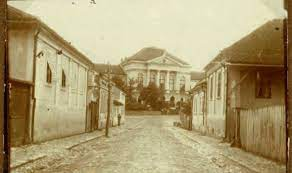
\includegraphics[height=3cm]{licej.jpg} 
        \caption{\emph{ Liceum u Kragujevcu}}
        \label{fig:liceum}
\end{figure}
 
\end{frame}

\subsection{Onlajn nastava}

\begin{frame}[fragile]\frametitle{Onlajn nastava}
	\begin{itemize}	
		\item Ubrzani razvoj onlajn nastave (uticaj pandemije)
		\item Diverzitet tipova nastave
        \item Kvalitet i efektivnost predavanja
		
	\end{itemize}
   \begin{figure}[h!]
        \centering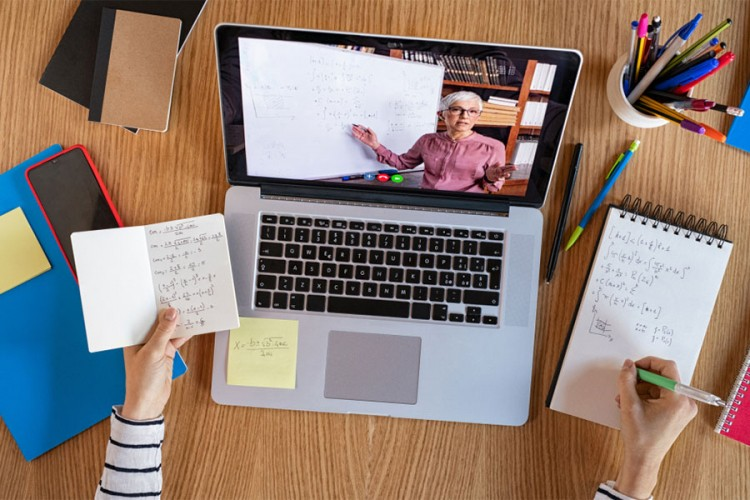
\includegraphics[height=3cm]{online1.jpg} 
        \caption{\emph{ Nastava kod kuće}}
        \label{fig:onlajn_nastava}
\end{figure}
\end{frame}


\subsection{Prednosti obrazovanja u Srbiji}
\begin{frame}[fragile]\frametitle{Prednosti obrazovanja u Srbiji}
\begin{itemize}
    \item Zastupljenost obrazovnih ustanova
    \item Bezbednost u školama
    \item Raznovrsnost fakulteta
    \item Način predavanja
\end{itemize}
\begin{figure}[h!]
        \centering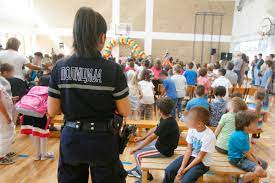
\includegraphics[height=3cm]{skolski_policajac.jpg} 
        \caption{\emph{ Školski policajac}}
        \label{fig:Bezbednost}
\end{figure}
\end{frame}



\subsection{Mane obrazovanja u Srbiji}
\begin{frame}[fragile]\frametitle{Mane obrazovanja u Srbiji}

\begin{itemize}
    \item Bezbednost
    \item Ocenjivanje učenika
    \begin{figure}[h!]
        \centering
        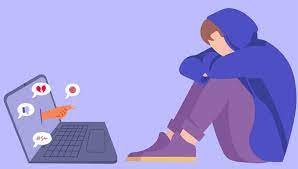
\includegraphics[height=3cm]{internet_nasilje.jpg} 
        \caption{\emph{ Internet nasilje}}
        \label{fig:Bezbednost}
\end{figure}
\end{itemize}

\end{frame}
\subsection{Poređenje sa ostatkom sveta}
\begin{frame}[fragile]\frametitle{Poređenje sa ostatkom sveta}

\begin{itemize}
    \item Srbija u poređenju sa:
    \begin{itemize}
        \item Zemljama istočne Azije
        \item  Estonijom
        \item Amerikom
    \end{itemize}

\end{itemize}

\end{frame}

\begin{frame}{Top 10}
\begin{table}[h!]
\begin{center}
\caption{Top 10 najobrazovanijih država(2018-OECD)}
\begin{tabular}{|c|l|} \hline
\textbf{država}& \textbf{\% obrazovanog stanovništva}\\ \hline
Kanada &56.27\\ \hline
Japan &50.50\\ \hline
Izrael &49.90\\ \hline
Južna Koreja &46.86\\ \hline
Velika Britanija &45.96\\ \hline
SAD &45.67\\ \hline
Australija &43.74\\ \hline
Finska &43.60\\ \hline
Norveška &43.02\\ \hline
Luksemburg &42.86\\ \hline
\end{tabular}
\label{tab:tabela1}
\end{center}
\end{table}
\end{frame}

\section{Zaključak}

\begin{frame}[fragile]\frametitle{Zaključak}
	\begin{itemize}
	    \item Srbija poseduje jak temelj školstva koji može samo da se unapredi, kako bi ostalim generacijama znanje bilo pristupačnije i proces učenja zanimljiviji.
        \item S obzirom da trenutno živimo u periodu ubrzanog razvoja tehnologije, treba maksimalno iskoristiti priliku i prilagoditi se što više savremenim metodama učenja.
	\end{itemize}
\end{frame}

\end{document}